\chapter{CONVERSORES PARA HTML}
\begin{draft}

Além da possibilidade de escrever em HTML, pode-se optar pela
alternativa de utilizar-se um conversor de linguagens.

\subsection{Bibliotecas relevantes do desenvolvimento de jogos}

Desenvolvedores da WEB são geralmente de mente aberta e desenvolveram
uma variedade de bibliotecas e frameworks pela internet \autocite{html5mostwanted}.

\cite{creatingFun} ressalta a importância de sermos moderados
quanto a escolha de bibliotecas no contexto WEB multiplataforma.
\begin{quote}
Muitos desenvolvedores da WEB utilizam bibliotecas como jQuery e o
Prototype de modo que se vejam livres de terem que lidar com
partes triviais do desenvolvimento WEB, como selecionar e
manipular elementos do DOM. Muitas vezes essas bibliotecas incluem
várias funcionalidades que não são utilizadas. É recomendável
cautela para verificar se realmente é necessário adicionar 50-100k
de bibliotecas, ou se alguma coisa mais simples e menor não trará
os mesmo benefícios, especialmente quando desenvolvendo
multiplataforma onde uma rápida conexão a internet nem sempre é
garantida.
\end{quote}

Esta preocupação aumenta no contexto de desenvolvimento de jogos.
Ainda segundo \cite{creatingFun} o site MicroJS https://microjs.com
oferece uma coleção de micro bibliotecas focadas em áreas
particulares em detrimento de grandes bibliotecas cheias de
funcitnalidades.

\section{Frameworks de jogos}

Com o intuito de simplificar o processo para os desenvolvedores,
auxiliando-os a focarem-se apenas nas soluções que estão
desenvolvendo, foram criados os frameworks para desenvolvimento de
jogos. Alguns frameworks reconhecidos são:

\begin{itemize}
\item enchant.js: dentre suas funcionalidades constam: orientação à, orientado à eventos, contém um motor de animação,
\item suporta WebGL e Canvas, etc three.js: considerada leve, renderiza, WebGL e Canvas, arquitetura procedural
\item limeJs: bom para 2d
\item quintus: especialista em jogos de plataforma 2D
\end{itemize}

\section{CROSSWALK}

Crosswalk empacota os fontes juntamente com uma versão do Chromium, a
versão Open-source do Google Chrome. Isso faz com que o software se
comporte da mesma forma para todas as versões de dispositivos Android.

\section{PHONEGAP}
\section{PHONEGAP CLOUD}

Este serviço possibilita que se faça upload de um arquivo compactado
contendo os fontes – ou apontando para um repositório no GitHub –
que no tempo desta pesquisa não estava funcionando; e se gere o APK
para o Android nativamente.

\section{NODEJS}

Permite rodar JavaScript fora do navegador. Utiliza um modelo dirigido
à eventos sem bloqueio, tornando-o rápido e eficiente.

\chapter{ALTERNATIVAS AO JAVASCRIPT}

Abaixo seguem algumas tecnologias que servem de alternativa ao
JavaScript.

\section{TYPESCRIPT}

Conhecido como uma versão estendida do JavaScript que compila para
JavaScript normal.

\section{DART}

Google. DartVM é uma máquina virtual que está embebido no Google
Chrome. Significante melhorias em performance quando comparado
ao JavaScript. Existe o dart2js que compila código em Dart para
JavaScript.

\chapter{SISTEMAS DE BUILDING}

Aquivos JavaScript são requisitados do servidor assincronamente. Isso
pode levar a tempos de requisição pouco desejáveis. Uma saída seria
escrever o código em apenas um arquivo mais isso leva a gerência de
código bagunçada. A saída mais comum entre desenvolvedores é utilizá
ruma ferramenta que junta todos os arquivos e disponibiliza apenas um
para o usuário.

Utiliza o conceito de streams para aplicar todas as modificações sobre
um arquivo de uma vez só.

\chapter{AMBIENTES PARA DESENVOLVIMENTO HTML5}

Na pesquisa efetuada sobre estes frameworks full-stack foram
identificadas as seguintes tecnologias:

Segundo \cite{gtw}
\begin{quote}
O GWT é um framework essencialmente para o lado do cliente (client
side) e dá suporte à comunicação com o servidor através de RPCs
(\textit{Remote Procedure Calls}). Ele não é um framework para
aplicações clássicas da web, pois deixa a implementação da
aplicação web parecida com implementações em desktop.
\end{quote}

Este é utilizado em muitos produtos de grande porte como o Google
Adwords e Google Wallet. Outra característica interessante é que a
plataforma opera sobre a licença Apache versão 2;

Construct 2 - é um editor na nuvem focado para usuários sem
    - conhecimento prévio em programação orientado a comportamento;
    - PlayCanvas - é uma plataformas para a construção de jogos 3D
na nuvem, desenvolvida com foco em performance. Permite a hospedagem,
controle de versão e publicação dos aplicativos nela criados,
possibilita também a importação de modelos 3D de softwares populares
como: Maya, 3ds Max e Blender;

    - o ambiente HTML5 da Intel, este fornece uma solução na nuvem,
completa para o desenvolvimento em plataforma cruzada, com serviços de
empacotamento, serviços para a criação e testes de aplicativos com
montagem de interfaces puxa e arrasta (Intel XDK) e bibliotecas para a
construção de jogos utilizando aceleração de hardware, o que garante
até duas vezes mais performance que aplicativos mobile baseados em
Web tradicionais. Esta solução é gratuita, open-source e funciona
através de um plugin para o Google Chrome, ou seja, o desenvolvimento
também é multiplataforma e devido ao fato de os binários ficarem
hospedados na nuvem, possibilitou a Intel criar compiladores para cada
uma das plataformas disponibilizadas pelo PhoneGap, que é o framework
polyfill utilizado na solução.

\chapter{METODOLOGIA DE DESENVOLVIMENTO DE SOFTWARE PARA A CONSTRUÇÃO DE GAMES}

Como o jogo é um software complexo demanda-se a utilização de
metodologias de engenharia de software, dentre os processos de software
mais conhecidos academicamente destacamos:

\begin{itemize}
\item OpenUP: este é bem detalhado e de característica iterativa e
incremental. Gerando assim, um levantamento mais apurado dos riscos,
requisitos e outros detalhes do sistema e a criação incremental do
sistema, com requisitos maleáveis;

\item Cascata: processo antigo, caracteriza-se por ser pouco maleável aos
requisitos mapeados posteriormente ao processo de análise;

\item  Processo ágil - SCRUM: sua utilização é flexível e sendo
um método ágil especifica pouca documentação, ou como dizem,
somente a documentação necessária, este processo é bem conhecido e
aceito na comunidade de desenvolvimento de software. Suas principais
características são: divisão do processo de desenvolvimento através
uma série de iterações chamadas sprints. Cada sprint consiste
tipicamente em duas a quatro semanas. É bem aplicado a projetos que
mudam constantemente e que demandam rápidas adaptações;

\item Processo ágil – XP: tem muitas características similares ao SCRUM
por este também ser um processo ágil. Dentre suas especifidades
destaca-se: versões frequentes, pequenos ciclos de desenvolvimento que
buscam aumentar a produtividade, introduzem checkpoints onde os clientes
podem agregar novas funcionalidades;
\end{itemize}

\end{draft}

\chapter{Diagrama de classes}
\begin{figure}
    \centering
    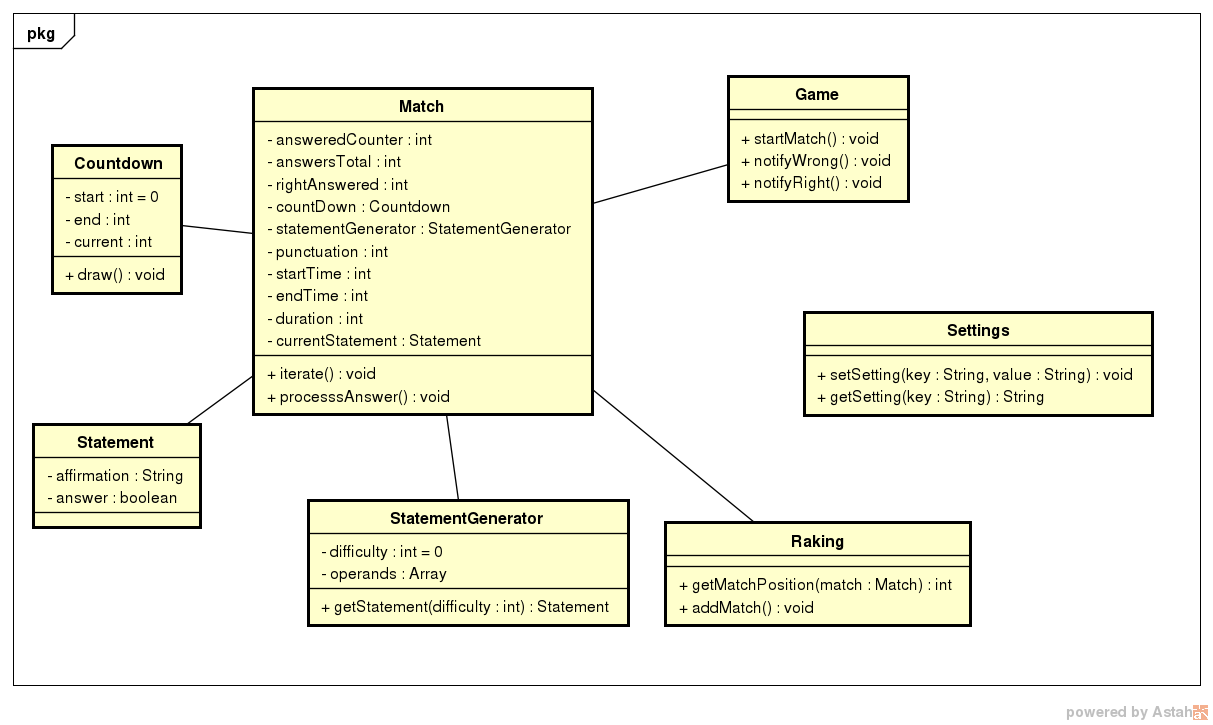
\includegraphics[width=0.8\textwidth,natwidth=610,natheight=642]{ClassesFullView.png}
	\caption{Diagrama de classes completo}
\end{figure}
